%@AUTHOR: Cardel
%Configuracion del documento

\documentclass{beamer}
\usetheme{Berkeley}
\setbeamertemplate{caption}[numbered]
\usepackage{graphicx}
\usepackage[utf8]{inputenc}
\usepackage[spanish]{babel}
\usepackage{ragged2e}
\usepackage{colortbl}
\usepackage{color}
\definecolor{naranja}{rgb}{1,0.5,0} % valores de las componentes roja, verde y azul (RGB)
\definecolor{rojo}{rgb}{1,0,0}
\definecolor{SteelBlue}{rgb}{0.3,0.5,0.7}
\usepackage{float}

\author{Carlos Andr\'es Delgado S.} 
\title{710193M Arquitectura de computadores II}
\subtitle{Aritmética del computador \\ carlos.andres.delgado@correounivalle.edu.co}
\institute{Facultad de Ingeniería. Universidad del Valle}
%Transparencia
\setbeamercovered{transparent}

%LOGO Univalle
\pgfdeclareimage[height=1.4cm]{logo}{imagenes/univalle}
\logo{\pgfuseimage{logo}}

\usepackage{listings}% http://ctan.org/pkg/listings
\usepackage{listingsutf8}

\lstset{ %
  basicstyle=\footnotesize,           % the size of the fonts that are used for the code
  numbers=left,
  numberstyle=\footnotesize,          % the size of the fonts that are used for the line-numbers
  numbersep=4pt,                  % how far the line-numbers are from the code
  backgroundcolor=\color{white},      % choose the background color. You must add \usepackage{color}
  breaklines=true,                % sets automatic line breaking
  breakatwhitespace=true,        % sets if automatic breaks should only happen at whitespace
  title=\lstname,                   % show the filename of files included with \lstinputlisting;{}
  extendedchars=false,
  inputencoding=utf8, 
  tabsize=2,
   mathescape=true,
  literate={\ \ }{{\ }}1
}
\newsavebox{\myLst}
\newsavebox{\myLstb}
\newsavebox{\myLstc}
\newsavebox{\myLstd}


%Para que en cada seccion aparezca la tabla de contenido
\AtBeginSection[]{
	\begin{frame}
	\frametitle{Contenido}
	\tableofcontents[currentsection]
\end{frame}
}



\date{Febrero de 2016}
\newcommand{\grad}{\hspace{-2mm}$\phantom{a}^{\circ}$}
\begin{document}

\begin{frame}
	\titlepage	 		
\end{frame}

\begin{frame}
	\tableofcontents	 		
\end{frame}
\section{Unidad lógica aritmética (ALU)}

\begin{frame}
	\frametitle{Unidad lógica aritmética}
	\begin{block}{Definiciones}
		\begin{itemize}
			\item Realiza cálculos aritméticos y lógicos
			\item Los elementos del computador suministra datos a la ALU
			\item Se basan en dispositivos lógicos digitales
		\end{itemize}
	\end{block}	
\end{frame}


\begin{frame}
	\frametitle{Unidad lógica aritmética}
	\begin{figure}[H]
	\centering
	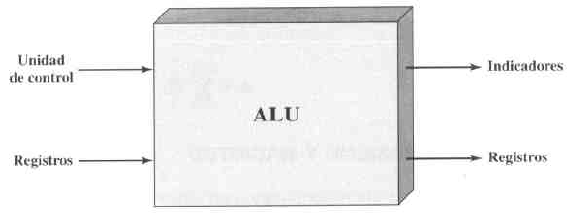
\includegraphics[scale=0.6]{imagenes/ALU.png}
	\caption{Entradas y salidas ALU}
	\end{figure}
	
\end{frame}


\section{Representación de enteros}

\begin{frame}
	\frametitle{Representación de enteros}
	\begin{block}{Definiciones}
		\begin{itemize}
			\item Cualquier número entero decimal puede representar en base binaria
			\item La base decimal consta de los dígitos $0,1,2,3,4,5,6,7,8,9$
			\item La base binaria consta de los dígitos $0,1$
		\end{itemize}
	\end{block}	
	\begin{exampleblock}{Ejemplo}
		
		\begin{center}
		$4_{10} = 100_{2}$
		\end{center}

	\end{exampleblock}
\end{frame}


\begin{frame}
	\frametitle{Representación de números reales}
	\begin{block}{Definiciones}
		\begin{itemize}
			\item Cualquier número real decimal se puede representar en binario
			\item Se debe tomar en cuenta la \textbf{coma de la base}
		\end{itemize}
	\end{block}	
	\begin{exampleblock}{Ejemplo}
		
		\begin{center}
		$10.025_{10} = 1010.01_{2}$
		\end{center}

	\end{exampleblock}
\end{frame}


\begin{frame}
	\frametitle{Representación de enteros}
	\begin{block}{Definiciones}
		\begin{itemize}
			\item Este tipo de representación sirve para que pueda ser procesada por el computador
			\item Si limitamos la representación a \textbf{número enteros no negativos} su representación es inmediata, si esta tiene $n$ bits se pueden representar números desde $0$ hasta $2^{n}-1$
		\end{itemize}
	\end{block}	
	\begin{exampleblock}{Ejemplo}
		Una palabra de 8 bits puede representar números entre 0 y 255 ejemplo:
		\begin{center}
			$00000000_{2}$ = $0_{10}$ \\
			$00010000_{2}$ = $16_{10}$ \\
			$10000000_{2}$ = $128_{10}$ \\
			$11111111_{2}$ = $255_{10}$
		\end{center}
	\end{exampleblock}
\end{frame}


\begin{frame}
	\frametitle{Representación de enteros}
	\begin{block}{Transformación decimal a binario}
		\begin{itemize}
			\item Para realizar la transformación de binario a decimal se realizan divisiones sucesivas por 2 y se toma el residuo
			\item Cuando se termina el proceso, el número en binario resultante es el orden inverso de los residuos
		\end{itemize}
	\end{block}	
	\begin{exampleblock}{Ejemplo}
		\begin{figure}[H]
			\centering
			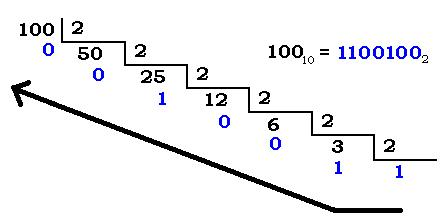
\includegraphics[scale=0.4]{imagenes/Conversion.jpg}
			\caption{Conversión decimal a binario}
			\end{figure}		
	\end{exampleblock}
\end{frame}


\begin{frame}
	\frametitle{Representación de enteros}
	\begin{block}{Ejercicio en clase}
	Transformar de decimal a binario los siguientes números:
		\begin{itemize}
			\item $1000_{10}$
			\item $2432_{10}$
			\item $175_{10}$
		\end{itemize}
	\end{block}	
\end{frame}



\begin{frame}
	\frametitle{Representación de enteros}
	\begin{block}{Ejercicio en clase}
	Respuestas:
		\begin{itemize}
			\item $1111101000_{2}$
			\item $100110000000_{2}$
			\item $10101111_{2}$
		\end{itemize}
	\end{block}	
\end{frame}

\begin{frame}
	\frametitle{Representación de enteros}
	\begin{block}{Transformación binario a decimal}
		\begin{itemize}
			\item Se toma en cuenta el valor de cada posición en base 2 y se multiplica por 0 o 1 según el caso
			\item Se suman estos valores para obtener el número en base decimal
		\end{itemize}
	\end{block}	
	\begin{exampleblock}{Ejemplo}
	\vspace{-0.3cm}
		\begin{figure}[H]
			\centering
			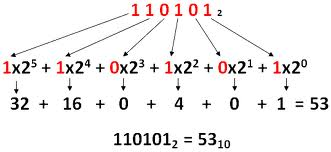
\includegraphics[scale=0.5]{imagenes/pasar-decimal-binario.jpg}
			\caption{Conversión binario a decimal}
			\end{figure}		
	\end{exampleblock}
\end{frame}

\begin{frame}
	\frametitle{Representación de enteros}
	\begin{block}{Ejercicio en clase}
	Transformar de binario a decimal los siguientes números:
		\begin{itemize}
			\item $10001011_{2}$
			\item $101101011011_{2}$
			\item $11101000110_{2}$
		\end{itemize}
	\end{block}	
\end{frame}

\begin{frame}
	\frametitle{Representación de enteros}
	\begin{block}{Ejercicio en clase}
	Respuestas:
		\begin{itemize}
			\item $139_{10}$
			\item $2907_{10}$
			\item $1862_{10}$
		\end{itemize}
	\end{block}	
\end{frame}


\begin{frame}
	\frametitle{Representación en suma magnitud}
	\begin{block}{Definición}
		\begin{itemize}
			\item Se utiliza para presentar enteros negativos y positivos
			\item El bit más a la izquierda (más significativo) es:
				\begin{enumerate}
					\item 1 si el número es negativo
					\item 0 si el número es positivo
				\end{enumerate}
			\item Para esta representación se establece el tamaño de $n$ bits, donde se utilizan $n-1$ bits para representar el número deseado
			\item El rango de representación en signo magnitud es $-2^{n-1}-1$ a $2^{n-1}-1$ para $n$ bits
		\end{itemize}
	\end{block}	
\end{frame}


\begin{frame}
	\frametitle{Representación en suma magnitud}

	\begin{exampleblock}{Ejemplo}
	Para el caso de $n=8$ se tiene por ejemplo:
		\begin{center}
			$18_{10} = 00010010_{2}$ \\
			$-18_{10} = 10010010_{2}$
		\end{center}
	\end{exampleblock}
\end{frame}


\begin{frame}
	\frametitle{Representación en suma magnitud}
	\begin{block}{Limitaciones}
		\begin{itemize}
			\item Existen dos representaciones del cero:
			\begin{enumerate}
				\item $0_{10} = 00000000_{2}$
				\item $0_{10} = 10000000_{2}$
			\end{enumerate}
			Esto es inconveniente ya que se tiene que tomar en cuenta las dos representaciones del cero
			\item Debido a la limitación de la representación en signo magnitud esta no es utilizada
		\end{itemize}
	\end{block}	
\end{frame}


\begin{frame}
	\frametitle{Representación en complemento a dos}
	\begin{block}{Definición}
		\begin{itemize}
			\item Se utiliza para presentar enteros negativos y positivos
			\item El bit más a la izquierda (más significativo) es:
				\begin{enumerate}
					\item 1 si el número es negativo
					\item 0 si el número es positivo
				\end{enumerate}
			\item Difiere en la forma de representar los bits restantes.
			\item El rango de la representación es: $-2^{n-1}$ hasta $2^{n-1}-1$
		\end{itemize}
	\end{block}	
\end{frame}


\begin{frame}
	\frametitle{Representación en complemento a dos}
	\begin{block}{Definición}
		Para calcular el complemento a dos de un número binario, se realiza el siguiente proceso:
		\begin{itemize}
			\item \textbf{Si es positivo:} Es la misma representación que signo magnitud
			\item \textbf{Si es negativo:} Aplique el siguiente procedimiento:
			\begin{enumerate}
				\item Cambie 0 por 1 y 1 por 0 a un número en representación de signo magnitud, excepto el bit más significativo
				\item Sume 1 al este número
			\end{enumerate}

		\end{itemize}
	\end{block}	
\end{frame}

\begin{frame}
	\frametitle{Representación en complemento a dos}
	\begin{exampleblock}{Ejemplo}
	Transforme 4 y -4 a signo magnitud, en una representación binaria de $4$ bits.
		\begin{enumerate}
			\item Para 4, en signo magnitud es: 0100, por lo que su representación en complemento a dos es 0100.
			\item Para -4, en signo magnitud es 1100, su complemento 1011 y lo sumamos 1, se obtiene 1100
		\end{enumerate}
	\end{exampleblock}
\end{frame}

\begin{frame}
	\frametitle{Representación en complemento a dos}
	\begin{block}{Ejercicio en clase}
	Transforme a complemento a dos los siguientes números decimales:
		\begin{itemize}
			\item $59_{10}$
			\item $-117_{10}$
			\item $207_{10}$
		\end{itemize}
	Suponga en todos los casos que se utiliza una representación de 10 bits.
	\end{block}	
\end{frame}

\begin{frame}
	\frametitle{Representación en complemento a dos}
	\begin{block}{Ejercicio en clase}
	Respuestas:
		\begin{itemize}
			\item $0000111011_{2}$
			\item $1110001011_{2}$
			\item $0011001111_{2}$
		\end{itemize}
	\end{block}
	\begin{block}{Enlace}
		Una herramienta útil: \url{http://www.exploringbinary.com/twos-complement-converter/}
	\end{block}		
\end{frame}


\section{Aritmética con enteros}

\begin{frame}
	\frametitle{Aritmética con enteros}
	\begin{block}{Negación}
		Para obtener el opuesto a un entero, se debe invertir los bits y sumarle 1.
	\end{block}	
	\begin{exampleblock}{Ejemplo}
	 	$18_{10} = 00010010_{2}$ \\
	 	Complemento bit a bit: $11101101_{2}$
	 	Sumandole 1: $11101110_{2} = -18_{10}$
	\end{exampleblock}
\end{frame}


\begin{frame}
	\frametitle{Aritmética con enteros}
	\begin{block}{Suma y resta}
		La suma y la resta se realiza en la misma forma como si los números fueran enteros sin signo.
	\end{block}	
	\vspace{-0.3cm}
	\begin{figure}[H]
		\centering
		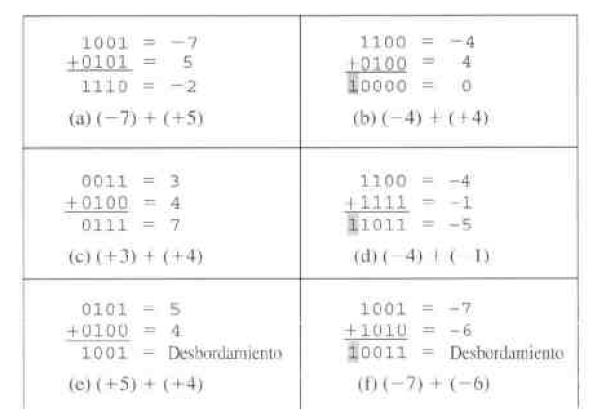
\includegraphics[scale=0.45]{imagenes/sumaresta.png}
		\caption{Suma de números en complemento a dos}
	\end{figure}
\end{frame}


\begin{frame}
	\frametitle{Aritmética con enteros}
	\begin{alertblock}{Regla de desbordamiento}
	Al sumar dos números, y ambos son o bien positivos o negativos, se produce desbordamiento si y sólo si el resultado tiene signo opuesto
	\end{alertblock}
	\begin{alertblock}{Regla de la resta}
	Para substraer un número (el substraendo) de otro (minuendo) se obtiene la negación del substraendo y se le suma al minuendo
	\end{alertblock}
\end{frame}


\begin{frame}
	\frametitle{Aritmética con enteros}
	\begin{figure}[H]
		\centering
		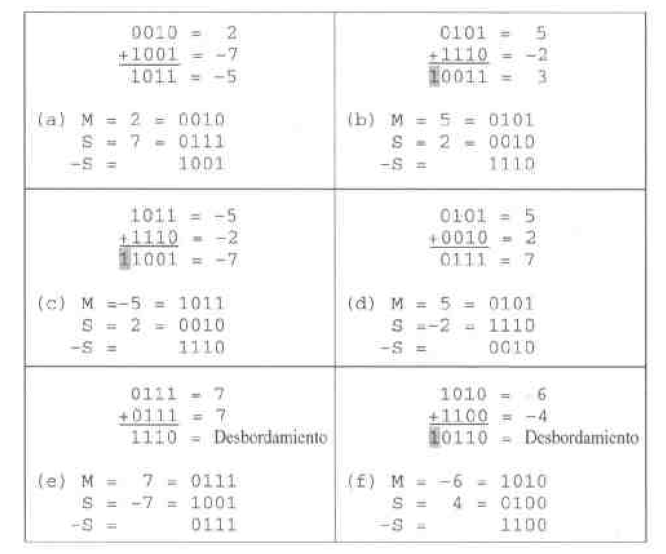
\includegraphics[scale=0.45]{imagenes/resta.png}
		\caption{Resta de números en complemento a dos}
	\end{figure}
\end{frame}


\begin{frame}
	\frametitle{Aritmética con enteros}
	\begin{figure}[H]
		\centering
		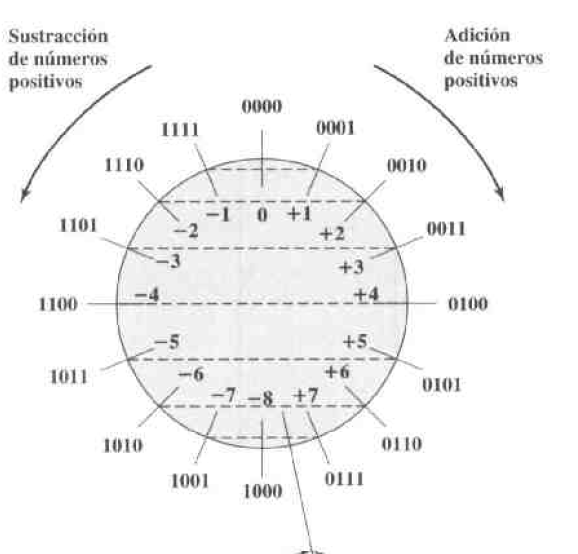
\includegraphics[scale=0.4]{imagenes/representacion.png}
		\caption{Representación suma y resta de números en complemento a dos}
	\end{figure}
\end{frame}


\begin{frame}
	\frametitle{Aritmética con enteros}
	\begin{block}{Multiplicación}
		La multiplicación es una operación compleja en hardware o software. En este caso se va discriminar la multiplicación entre enteros con y sin signo
	\end{block}	
	\begin{block}{Multiplicación enteros sin signo}
		Es similar a la multiplicación clásica.
	\end{block}	
\end{frame}

\begin{frame}
	\frametitle{Aritmética con enteros}
	\begin{figure}[H]
		\centering
		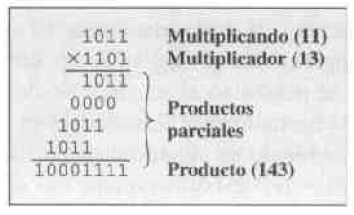
\includegraphics[scale=0.7]{imagenes/multiplicacion.png}
		\caption{Multiplicacion enteros sin signo}
	\end{figure}
\end{frame}

\begin{frame}
	\frametitle{Aritmética con enteros}
	\begin{block}{Multiplicación enteros con signo}
		Para los enteros con signo se utiliza la notación de complemento a dos. Debido a que esta no es sencilla se utiliza la representación de un número binario en potencias de dos:
	\begin{figure}[H]
		\centering
		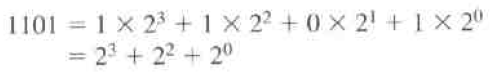
\includegraphics[scale=0.4]{imagenes/representaciondecimal.png}
		\caption{Representación de un número como suma de potencias}
	\end{figure}
	Por lo que se puede realizar la multiplicación en complemento a dos como sumas de multiplicaciones parciales.
	\end{block}	
\end{frame}


\begin{frame}
	\frametitle{Aritmética con enteros}
	\begin{block}{Multiplicación enteros con signo}
	\begin{figure}[H]
		\centering
		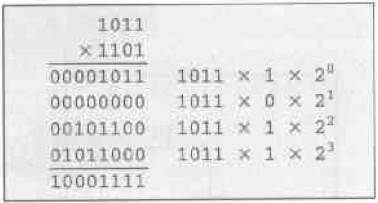
\includegraphics[scale=0.6]{imagenes/multiplica.png}
		\caption{Ejemplo multiplicación en complemento a dos}
	\end{figure}
	\end{block}	
\end{frame}

\begin{frame}
	\frametitle{Representación en complemento a dos}
	\begin{block}{Ejercicio en clase}
	Realiza las siguientes multiplicaciones.
		\begin{itemize}
			\item $5_{10} * -10_{10}$
			\item $4_{10} * -16_{10}$
			\item $-15_{10} * -3_{10}$
		\end{itemize}
	Suponga en todos los casos que se utiliza una representación de 8 bits.
	\end{block}	
\end{frame}

\begin{frame}
	\frametitle{Aritmética con enteros}
	\begin{block}{División}
		La división es una operación altamente costosa, en nuestro caso se realiza de igual forma que la división clásica.
	\begin{figure}[H]
		\centering
		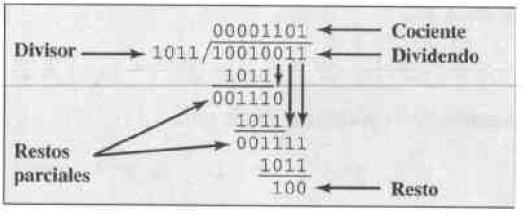
\includegraphics[scale=0.6]{imagenes/division.png}
		\caption{Ejemplo división enteros sin signo}
	\end{figure}
	\end{block}	
\end{frame}

\begin{frame}
	\frametitle{Preguntas}
	\vfill
	\begin{center}
	¿Preguntas?\\
	\vfill
	Siguiente clase: \\
	Aritmética del computador:\\
	Representación y aritmética en coma flotante
	\end{center}
\end{frame}



\end{document}